\chapter{ Challenges and Annotation Language Extension}
\section{Challenges and Idea}
Previous annotation language grammer has been extended more
to detect implicit and explicit information flow bugs in UML
state charts and C code. The purpose of the same annotation language
can be used to add information flow constraints to UML state
charts and code in order to detect information flow errors.\\

The challenge was addressed by extending the annotation language containing textual annotations which can be used to annotate source code and UML state charts which are backward compatible.The single-line annotations have the same as previous consisting start tag "//@" and the multi-line annotations have the start tag "/*@" and the end tag "@*/" .\\

Some challenges throughout the approach are- converting textual
comments into annotations objects, introducing syntactically
correct annotations into files, how to use the same annotation
language in order to annotate UML state charts and source
code, dealing with scattered annotations and attaching annotations to the right function declaration or variable.\\

The xText based grammar is used to parse the whole C/C++ language. The C/C++ source code file extensions (.h, .hh, .hhh, .hxx, .c, .cpp) and UML state chart annotation box (graphical boxes
which can be attached to different parts of a UML state chart diagram) can be annotated with policy language restrictions. The obtained CORE model (a one to one mapping from xText grammar to the ECORE grammar representation) that can be reused for integrating the policy language into an UML state chart editor. Treating the annotation tags as EObjects created new possibilities for annotating
UML models.The policy language grammar has about 400 LOC with code comments included. Source code generation is also supported by using
xTend, ANTLR and .mwe2 files. To parse other programming languages as well this annotation language parser can be used.The result is an extensible policy language and a highly reusable source code implementation that can easily be used for annotating models and source files.

\section{Annotation Language Tags}


\section{Language Implementation Process}

The process depicted in figure 3.1 was used in order to
implement annotation language. Figure 3.1 depicts the
annotation language implementation process. The process is
comprised of the following steps: At first, the .xtext file
containing the language grammar was extended following the requirements. Next the grammar file is compiled and software
artifacts are generated. After editing the .mwe2 file then compile it. The result of compiling is: a parser, a lexer and class bindings between these two (lexer and parser) and the grammar ECore model. The generated parser, lexer and the bindings were reused inside static analysis engine and in the UI source file editor. After opening and editing a source file with the editor,the file can be parsed and the annotations can be automatically loaded and used inside checkers.
\begin{figure}[htbp]
	\centering
	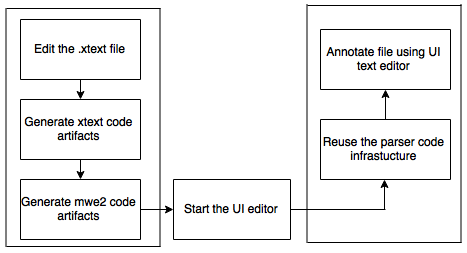
\includegraphics{styles/Language_Design_Process.png}
	\caption{Annotation language design process}
\end{figure}